\documentclass{article}
\usepackage[hidelinks]{hyperref}
\usepackage{csquotes}
\usepackage[vmargin=30mm, hmargin=30mm]{geometry}
\usepackage{amsmath}
\usepackage{xcolor}
\usepackage{listings}
\lstset{
    backgroundcolor=\color[RGB]{240, 240, 240},   
    basicstyle=\ttfamily\footnotesize,
    breakatwhitespace=false,
    breaklines=true,
    %    captionpos=b,
    keepspaces=true,
    numbers=left,
    numbersep=5pt,
    showspaces=false,
    showstringspaces=false,
    showtabs=false,
    tabsize=4,
    postbreak=\mbox{\textcolor{red}{$\hookrightarrow$}\space}
}

\lstdefinelanguage{docker}{
  keywords={FROM, RUN, COPY, ADD, ENTRYPOINT, CMD,  ENV, ARG, WORKDIR, EXPOSE, LABEL, USER, VOLUME, STOPSIGNAL, ONBUILD, MAINTAINER, HEALTHCHECK},
  keywordstyle=\color{blue}\bfseries,
  identifierstyle=\color{black},
  sensitive=false,
  comment=[l]{\#},
  commentstyle=\color{purple}\ttfamily,
  stringstyle=\color{red}\ttfamily,
  morestring=[b]',
  morestring=[b]"
}

% \usepackage{longtable}
% \usepackage{array}
\usepackage[
    backend=biber,
    sorting=none,
    style=ieee,
    urldate=long,
    maxcitenames=2,
    mincitenames=1
]{biblatex}
\addbibresource{sources.bib}
\usepackage{multicol}
\setlength{\columnsep}{13mm}
\usepackage{float}
\usepackage{graphicx}
\usepackage{caption}
\captionsetup{justification=centerlast,font=small,labelfont=sc,margin=50pt}


\let\savedCite=\cite
\renewcommand{\cite}{\unskip~\savedCite}
\let\savedRef=\ref
\renewcommand{\ref}{\unskip~\savedRef}
\hfuzz=50px
\hbadness=10000

\title{Running KLEE on GNU coreutils}

\begin{document}

\author{%
    Valentin Huber\vspace{5px}\\%
    \small \href{https://www.zhaw.ch/en/engineering/institutes-centres/init/}{Institute of Applied Information Technology}\\%
    \small \href{https://www.zhaw.ch/en}{Zürich University of Applied Sciences ZHAW}\\%
    \small \href{mailto://contact@valentinhuber.me}{contact@valentinhuber.me}%
    \vspace{10px}
}

\date{\today\vspace{5px}}

\maketitle

\tableofcontents

\section{Introduction}
KLEE\cite{KLEEWebsite} is an open source, symbolic execution based, advanced fuzzing platform. It was introduced in the seminal paper titled \citetitle{KLEE} in \citeyear{KLEE}. In their article, \citeauthor{KLEE} present their work and evaluate it on a diverse set of programs. The most prominent of those is the GNU coreutils suite, in which ten fatal errors were found.

Ever since then, KLEE has not only matured as a fuzzer, it has also been used extensively as a platform for other researchers to build on top of, as I have discovered in\cite{EVA}. As an introduction to the practical side of fuzzing, I attempted to answer the following questions about KLEE:

\begin{enumerate}
    \item Reproducing the original paper (see Section~\ref{Reproducing})
          \begin{enumerate}
              \item Can the current version of KLEE be run on coreutils version 6.10 (as tested in the original paper)?
              \item Can the same metrics as measured in the original paper still be measured?
          \end{enumerate}
    \item Examining the statistical distribution of results over different fuzzing times (see Section~\ref{Timeouts})
          \begin{enumerate}
              \item How does the non-determinism in KLEE influence the variance in the results between different test runs?
              \item How do the measured metrics compare to what was published 15 years ago?
              \item How do different testing timeouts influence results?
          \end{enumerate}
    \item Testing more recent versions of coreutils (see Section~\ref{SoftwareEvolution})
          \begin{enumerate}
              \item What needs to change in the test setup to test more recent versions of coreutils?
              \item How do the results from testing different versions of coreutils differ?
          \end{enumerate}
\end{enumerate}

All experiments were run on a virtualized server with the following specs: AMD EPYC 7713 64C 225W 2.0GHz Processor, 1 TiB RAM, 2x 25GiB/s Ethernet.
\section{Background}

What follows is a short explanation of the application of symbolic execution in fuzzing. For more extensive background, I refer to some of my previous work\cite{EVA, BA}.

Remember that KLEE is an open-source, symbolic execution based fuzzer. It takes LLVM bytecode from the program under test (PUT) as its input, runs its analysis on it. KLEE then outputs some statistics about the run, inputs to the PUT that crash it, and inputs that, when executed, cover all branches KLEE has examined during its analysis.

\subsection{A Primer on Symbolic Execution}
KLEE is a fuzzer based on symbolic execution. This means that instead of executing a PUT with a concrete value, it instead runs through the instructions and maps relationships between data in memory (such as variables and user input) to mathematical formulas. So an instruction like \lstinline[language=llvm]{%result = add i32 %a, %b} would be mapped to the logical relationship $\phi_k=\phi_i+\phi_j$. Conditional jumps are mapped to conditions on these variables for both outcomes of the condition, so the instruction \lstinline[language=llvm]{%isPositive = icmp sgt i32 %result, 0} would be represented with $\phi_k>0$ and $\phi_k\le0$ respectively.

The set of all conditions along a certain path through the PUT are called the \textit{path condition}. It can be passed to s satisfiability modulo theories (SMT) solver (KLEE uses STP\cite{STP} as a default), which returns values for all user inputs, such that the PUT is forced down the exact path represented by the path condition.

This is the major advantage of symbolic execution based fuzzing, as compared to ordinary fuzzing. By not using concrete values, but instead logical representations of user input, it essentially runs through the PUT with all possible user inputs \textit{at the same time}. So if the solver returns that no inputs satisfy the passed formula, we have proven that such inputs simply do not exist. To be able to do this, it accepts the huge overhead of translating the code to formulas and then solving them.

\subsection{Symbolic Execution in Practice}
\label{SymbexPractice}
Symbolic execution in fuzzing has several major challenges to overcome. I have previously discussed them in detail\cite{EVA}, but would like to give a short summary here:

\begin{itemize}
    \item Environment interactions (such as file system interactions) in general are opaque to the fuzzer and cannot be mapped to logical formulas. KLEE deals with this by solving the path constraint before the instruction in question and then uses concrete values in the call. This abandons the claim on completeness symbolic execution typically has, but is often the only feasible way to still continue analysis.
    \item The second major challenge in symbolic execution is what is known as \textit{path explosion}. Because the number of program states grows exponentially with the number of instructions, for all but the most simple programs it is not feasible to calculate the entire state space. KLEE deals with this by reducing the search space to actually executable instructions, using advanced data structures, and examining paths through the PUT consecutively, with a user-defined timeout. To maximize the state space and code coverage as quickly as possible, it alternates between two strategies for choosing the next input to evaluate: KLEE either chooses the input that promises to increase the coverage the most and a random input to prevent the execution from getting stuck in a certain subtree of the PUT.
    \item KLEE needs to model the entire memory of a process. This is straight-forward as long as variables are used directly but becomes a challenge when pointers are involved. This is especially true if the value of these pointers depends on user input, since this would require KLEE to model all possible addresses having all possible values, which instantly explodes the memory consumption and number of states to examine and is thus infeasible. KLEE deals with this by representing such pointer operation as array accesses where the accessed object is copied as often as necessary to model all possible results, including error states.
    \item As programs become more complex, the path constraints become increasingly long and solving them contributes more and more to the fuzzer's runtime. KLEE applies some advanced optimizations, like query splitting and more general optimizations, or a cache of previous results, which often solve supersets the query they are a solution to. Finally, KLEE defines a timeout, after which the solver is interrupted and analysis is continued at an other branch.
\end{itemize}

\section{Reproducing the Original Paper}
\label{Reproducing}
I'm basing my experiment setup on the original paper\cite{KLEE}, the FAQs in the project's documentation\cite{KLEEFAQ} and the tutorial on testing coreutils version 6.11\cite{KLEETutorial}.

\subsection{Project Setup}
\label{ProjectSetup}
KLEE is a complex system including complex dependencies such as the SMT solvers. The maintainers provide a Dockerfile and the corresponding Docker image. Using Docker as an intermediate form of virtualization adds a layer of indirection and a performance penalty. However, since I'm not necessarily interested in maximizing performance in this project, but instead focus on comparing different setups, this is a tradeoff worth taking. Using Docker to evaluate fuzzers' performance has been done before\cite{UNIFUZZ}. Finally, this makes complex build steps reproducible and acts as documentation.

\subsection{Naïve Approach}

When attempting to build coreutils 6.10 directly in the current version of KLEE's Docker image, I ran into an issue: The Docker image is based on Ubuntu 22 (Jammy), and no longer is able to build coreutils 6.10 with the GNU Compiler (GCC). This is because coreutils' build system attempts to detect what system it is running on, and the variable the detection is based on is no longer defined. Specifically, in \lstinline{freadahead.c} the following check is performed:

\lstinputlisting[
    firstline=25,
    lastline=25,
    language=C,
    consecutivenumbers=false
]{assets/freadahead.c}

The error message and the full \lstinline{freadahead.c} can be found in Appendix~\ref{AppendixErrorBuildOldInNew}.

\subsection{Using an Old Version of Ubuntu}
\label{OldVersion}

One attempt to mitigate this issue would be to rewrite this check to allow the version of GCC installed on KLEE's Docker image to compile coreutils 6.10. However, I opted to pursue a different avenue, because of two reasons:
\begin{enumerate}
    \item Build systems are not my area of expertise and I do not know how many other issues would appear once the first was solved.
    \item Changing code always adds risk of introducing additional software errors, which would distort my findings.
\end{enumerate}

Therefore, I attempted to build the binaries on an old version of Ubuntu, and then move the binaries to KLEE's Docker image. Specifically, I chose the latest LTS version which was available when version 6.10 of coreutils was current. This approach worked without any additional changes to the code nor the build system. The setup of the Docker image then used to build coreutils can be seen in Listing~\ref{dockerfile1}.

\lstinputlisting[
    float,
    language=docker,
    lastline=21,
    consecutivenumbers=false,
    caption=Dockerfile content to prepare a system for building coreutils 6.10,
    label=dockerfile1
]{../Dockerfile}

\subsection{Generating LLVM Bytecode Files}
\label{LLVM}

Building binaries themselves is unfortunately not enough, since KLEE does not take pure binaries as its input, but instead requires LLVM bytecode. Compiling an ordinary \lstinline{.c} file to LLVM can easily be done using \lstinline{clang}. However, again, coreutils use a complex build system which means to just use \lstinline{clang}, I'd have to deeply understand and modify it, with the drawbacks listed above.

Simply passing \lstinline{clang} as the C compiler to the build system does not work, since the produced output is not a runnable binary, and the build system requires the compiler's output to be executable.

Fortunately, there exists Whole Program LLVM (WLLVM)\cite{WLLVM}, a tool specifically designed to work with complex build systems while still producing LLVM bytecode as one of its outputs. This is achieved by injecting its compiler into the build system. The compiler creates executable binaries and additionally injects LLVM bytecode into a dedicated section of the object files. In a second step, these then get extracted and linked together to produce LLVM bytecode files.

Since I'm running WLLVM on an old version of Ubuntu, I was forced to use an old version of WLLVM as well, because newer versions require a version of python which is not available on Ubuntu 14.04. To create proper input files for KLEE, I added two options, to reduce warnings (\lstinline{--build}) and to turn off premature optimizations according to the KLEE documentation (\lstinline{CFLAGS})\cite{KLEETutorial}.

The Dockerfile section to build the LLVM bytecode can be found in Listing~\ref{dockerfile2}.

\lstinputlisting[
    float,
    language=docker,
    firstline=23,
    lastline=54,
    consecutivenumbers=false,
    caption=Dockerfile content to build coreutils to LLVM bytecode using WLLVM,
    label=dockerfile2
]{../Dockerfile}

\subsection{Coverage Data Gathering}
\label{gcov}

A simple way to compare what these experiments accomplish compared to the experiments documented in the original paper is to look at coverage data, specifically coverage as measured by \lstinline{gcov}. To gather this information, one needs to compile the binaries using GCC, and tell the compiler to add coverage gathering instrumentation. Along with the binaries, a note document (\lstinline{<executable-name>.gcno}) is created. When the binary is executed, the added instrumentation records which path through the code is taken and, together with information from the notes file, stores its results in a coverage data file (\lstinline{<executable-name>.gcda}). This file can then be analyzed with \lstinline{gcov} to get human-readable coverage data.

With this step however, I ran into the same issue as before: Recent versions of GCC no longer build coreutils 6.10. I adopted the same approach and used the same base image as described in Section~\ref{OldVersion}. The Dockerfile excerpt with the build step can be found in Listing~\ref{dockerfile3}.

\lstinputlisting[
    float,
    language=docker,
    firstline=56,
    lastline=70,
    consecutivenumbers=false,
    caption=Dockerfile content to build coreutils instrumented to record coverage,
    label=dockerfile3
]{../Dockerfile}

I made two changes compared to building the LLVM bytecode files, to increase the accuracy of the measurements:
\begin{itemize}
    \item I replaced all calls to \lstinline{_exit} with calls to \lstinline{exit}, so that those instructions are also included in the measurements. This was done according to the instructions in the FAQ\cite{KLEEFAQ}.
    \item The original paper mentions that coverage is measured only on executable lines of code. Specifically, Section 5.1 of the original paper says
          \begin{displayquote}
              \textquote{We measure size in terms of executable lines if code (ELOC) by counting the total number of executable lines in the final executable after global optimization, which eliminates uncalled functions and other dead code.}\cite{KLEE}
          \end{displayquote}
          I am not sure how \citeauthor{KLEE} calculated the executable lines of code, since this is not trivial. I did enable normal global optimization (\lstinline{-O2}), but this may still result in a considerable underestimation of coverage.
\end{itemize}

\subsection{Preparing KLEE}

Finally, the bytecode files can be passed to KLEE for the actual fuzzing. To prepare KLEE's Docker image, the environment and sandbox are prepared according to the documentation\cite{KLEEFAQ}. Then, the bytecode files from the step outlined in Section~\ref{LLVM} and the binaries instrumented with \lstinline{gcov} along with their notes files are copied to the analysis image. The analysis step itself is an involved process itself and is done by executing a shell script (\lstinline{analyze.sh}). This step is explained in Section~\ref{analyze.sh}. The analysis script is copied into the image and executed on container start. To allow passing certain settings to the analysis step, environment variables are used,which can be set in the \lstinline{docker run} command.

The Dockerfile excerpt for this step can be found in Listing~\ref{dockerfile4}.

\lstinputlisting[
    float,
    language=docker,
    firstline=84,
    lastline=117,
    consecutivenumbers=false,
    caption=Dockerfile content to prepare the fuzzing stage,
    label=dockerfile4
]{../Dockerfile}

\subsection{Running KLEE}
\label{analyze.sh}
When starting the Docker image built with the steps outlined before, a shell script is executed. This script handles the evaluation settings, input and output files, and collects metrics. Specifically, the following steps are performed:

\begin{enumerate}
    \item The input including the passed settings are parsed. The script allows setting input and output directories (\lstinline{--llvm-dir}, \lstinline{--cov-dir}, \lstinline{--out-dir}), KLEE's timeout (\lstinline{--klee-max-time}), and skipping the fuzzing step (\lstinline{--skip-klee-analysis}). The latter allows gathering additional metrics without based on the output from a previous fuzzing run without having to perform additional, computationally expensive analysis.
    \item To run KLEE, the analyst is required to pass arguments setting the size and number of inputs and input files to be tested. For most coreutils, this is the same, however (as mentioned in Section 5.2 of the original paper\cite{KLEE} and explained in the FAQs\cite{KLEEFAQ}) some utils need different settings to achieve a decent coverage. The analysis script assembles the command to run KLEE, including the constant settings, util-dependant settings, and the timeout set in the script arguments.
    \item Then, the actual fuzzing is performed.
    \item KLEE's output is examined in a few ways:
          \begin{enumerate}
              \item For each found error, human readable outputs are created using \lstinline{ktest-tool}.
              \item \lstinline{klee-stats} is invoked to export metrics collected by KLEE.
              \item All test cases generated by KLEE are used as input for \lstinline{klee-replay} pointed at the binary instrumented with coverage gathering instructions. This ensures that each instruction analyzed by KLEE during its fuzzing is also executed and thus recorded in the coverage results. Since the instrumented binaries were not compiled on the same system as they are executed on, the environment variables \lstinline{GCOV_PREFIX} and \lstinline{GCOV_PREFIX_STRIP} need to be set appropriately.
          \end{enumerate}
    \item Finally, certain large output text files are compressed to minimize disk usage.
\end{enumerate}

\subsection{Extracting Human-Readable Coverage Data}

As a last step, the output of the binaries instrumented to gather coverage metrics needs to be fed back into \lstinline{gcov}. Unfortunately, the format of these output files changed at some point and the version of \lstinline{gcov} installed in KLEE's Docker image is no longer able to read them. They are therefore fed back into the Docker image that created them, where an obviously compatible version of \lstinline{gcov} is available.

\subsection{Gathered Metrics}

In each run on each util of the experiment as discussed above, the following metrics were collected:

\begin{itemize}
    \item The util name including the version and the run
    \item The timeout passed to KLEE
    \item The number of errors as reported by KLEE by type according to the file extension:
          \begin{itemize}
              \item \lstinline{ptr} errors, e.g. invalid pointers, null page accesses, out of bound pointers
              \item \lstinline{exec} errors, which appear on illegal instructions and external calls with a symbolic \lstinline{errno} call
              \item \lstinline{model} errors, which appears when a symbolic size is concretized
              \item \lstinline{solver} errors, which are query timeouts
              \item \lstinline{abort} errors
              \item The total number of errors
          \end{itemize}
    \item Instruction and branch coverage\footnote{KLEE includes library code in its coverage numbers, and thus reports significantly lower coverage compared to \lstinline{gcov}.} as reported by KLEE\footnote{KLEE reports a set of additional metrics like time spent in the solver, number of instructions analyzed and number of cache hits, but these were not examined further in this paper.}
    \item Coverage as measured by \lstinline{gcov}
\end{itemize}
\section{Comparing Runs}
\label{Timeouts}

Figure~\ref{fig:spread_60min_6.10} shows the spread of the measurements between four runs of the experiments with the same parameters. The non-deterministic nature of the results is due to the inherent non-determinism of the fuzzing process in KLEE (refer to Section~\ref{SymbexPractice}). Specifically, the standard deviations for code coverage by branch (according to KLEE), instruction (according to KLEE) and line (according to \lstinline{gcov}) are 0.37\%, 0.48\%, and 1.56\% respectively.

\begin{figure}[hb]
    \centering
    \includegraphics[width=1\textwidth]{assets/spread_60min_6.10.png}
    \caption{Spread of values normalized to the mean by util for coreutils 6.10 and a timeout of 60 minutes}
    \label{fig:spread_60min_6.10}
\end{figure}

Purely looking at the number of errors in each category is a very broad and imprecise way of measuring results. However, comparing and deduplicating errors found by a fuzzer is an art in itself, and simple approaches like comparing stack traces or the paths taken through software are insufficiently precise. The only accurate way to estimate the number (and severity) of errors is to manually look for the defect in the source code and compare the logic errors leading to the different findings.\cite{EvaluatingFuzzTesting} This is a lengthy task and requires intimate knowledge of the software under test and was thus declared out of scope for this project.

\subsection{Comparison to the Original Paper}

Figure~\ref{fig:KLEE_ecdf} is taken from the original KLEE paper\cite{KLEE} and shows the empirical cumulative distribution function (ECDF) of the coverage measured in their experiments. Figure~\ref{fig:ecdf_60min_6.10} shows the same measurements from the four runs done with the same settings as in the original paper.

It is important to note that the settings proposed by the documentation\cite{KLEEFAQ} do not include failing system calls, thus need to be compared to \textquote{Base} (white) elements of the graph in Figure~\ref{fig:KLEE_ecdf} only.

In general, Figures~\ref{fig:KLEE_ecdf} and~\ref{fig:ecdf_60min_6.10} do look reasonably similar, validating the approach taken in this paper.

However, there clearly is a difference visible between the two graphs, namely that the results I was able to achieve lag behind those reported in the original paper. Since discrete numbers from the original paper unfortunately are not available, and guessing results from a graph with mediocre resolution is error-prone, further numerical analysis of this difference is not performed. From looking at the variance in the four runs in Figure~\ref{fig:ecdf_60min_6.10}, it seems unlikely that the difference is purely statistical.

I do not have a definitive answer for the discrepancies, but the explanation might include differences in measurements, specifically in the calculation of executable lines of code (as discussed in Section~\ref{gcov}), changes in the version of KLEE the original experiments were performed with and the current version of KLEE, and performance differences between the machines the experiments were run on. The latter would either require that the performance penalty incurred by using Docker is greater than the speedup gained by 15 years of hardware developments or be based on bottlenecks during the experiments, such as I/O bandwidth.

\begin{figure}[ht]
    \centering
    \begin{minipage}[b]{0.48\linewidth}
        \includegraphics[width=\linewidth]{assets/KLEE_ecdf.png}
        \captionsetup{width=0.7\linewidth, skip=24px}
        \caption{Coverage according to the original KLEE paper\cite{KLEE}}
        \label{fig:KLEE_ecdf}
    \end{minipage}
    \hfill
    \begin{minipage}[b]{0.48\linewidth}
        \includegraphics[width=\linewidth]{assets/ecdf_60min_6.10.png}
        \captionsetup{width=0.75\linewidth}
        \caption{Coverage measured by \lstinline{gcov} across four runs}
        \label{fig:ecdf_60min_6.10}
    \end{minipage}
\end{figure}

\subsection{Influence of Timeout}

The performance drawbacks resp. benefits of my testing setup can be indirectly measured by changing the timeout passed to KLEE. This experiment was further inspired by the seminal work by~\citeauthor{EvaluatingFuzzTesting}, who collected a series of guidelines that should be followed to accurately measure the performance of a fuzzer. They propose that multiple runs should be performed to increase accuracy and found that \textquote{longer timeouts may be needed to paint a complete picture of an algorithm's performance}\cite{EvaluatingFuzzTesting}.

I chose three additional durations to conduct experiments at, with a large enough difference to ensure a complete picture of KLEE's performance across durations: 10 minutes, 6 hours and 24 hours.

\subsubsection{Changes in Coverage}

Figure~\ref{fig:ecdf_across_times} shows the ECDF of at least three runs across the different timeouts. Predictively, the coverage increases with increased timeouts. The difference between the timeouts does not seem too big, and this is confirmed by Figure~\ref{fig:spread_across_times_gcov}.


\begin{figure}[ht]
    \centering
    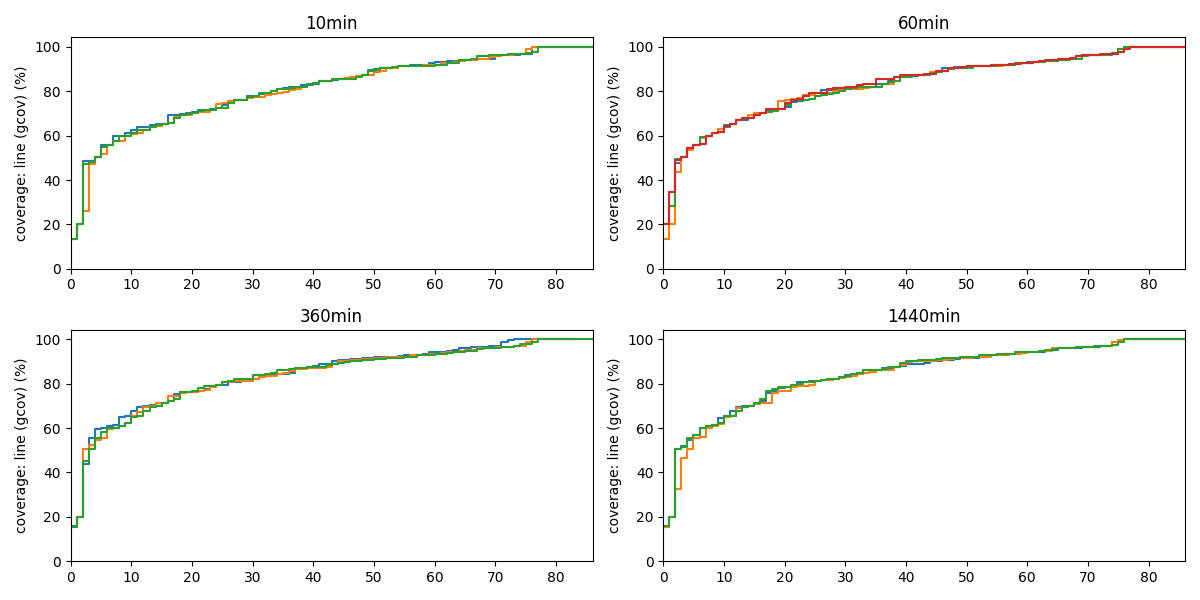
\includegraphics[width=1\textwidth]{../plots/gcov_cov/ecdf_by_time.png}
    \caption{Coverage measured by \lstinline{gcov} across different timeouts}
    \label{fig:ecdf_across_times}
\end{figure}

\begin{figure}[ht]
    \centering
    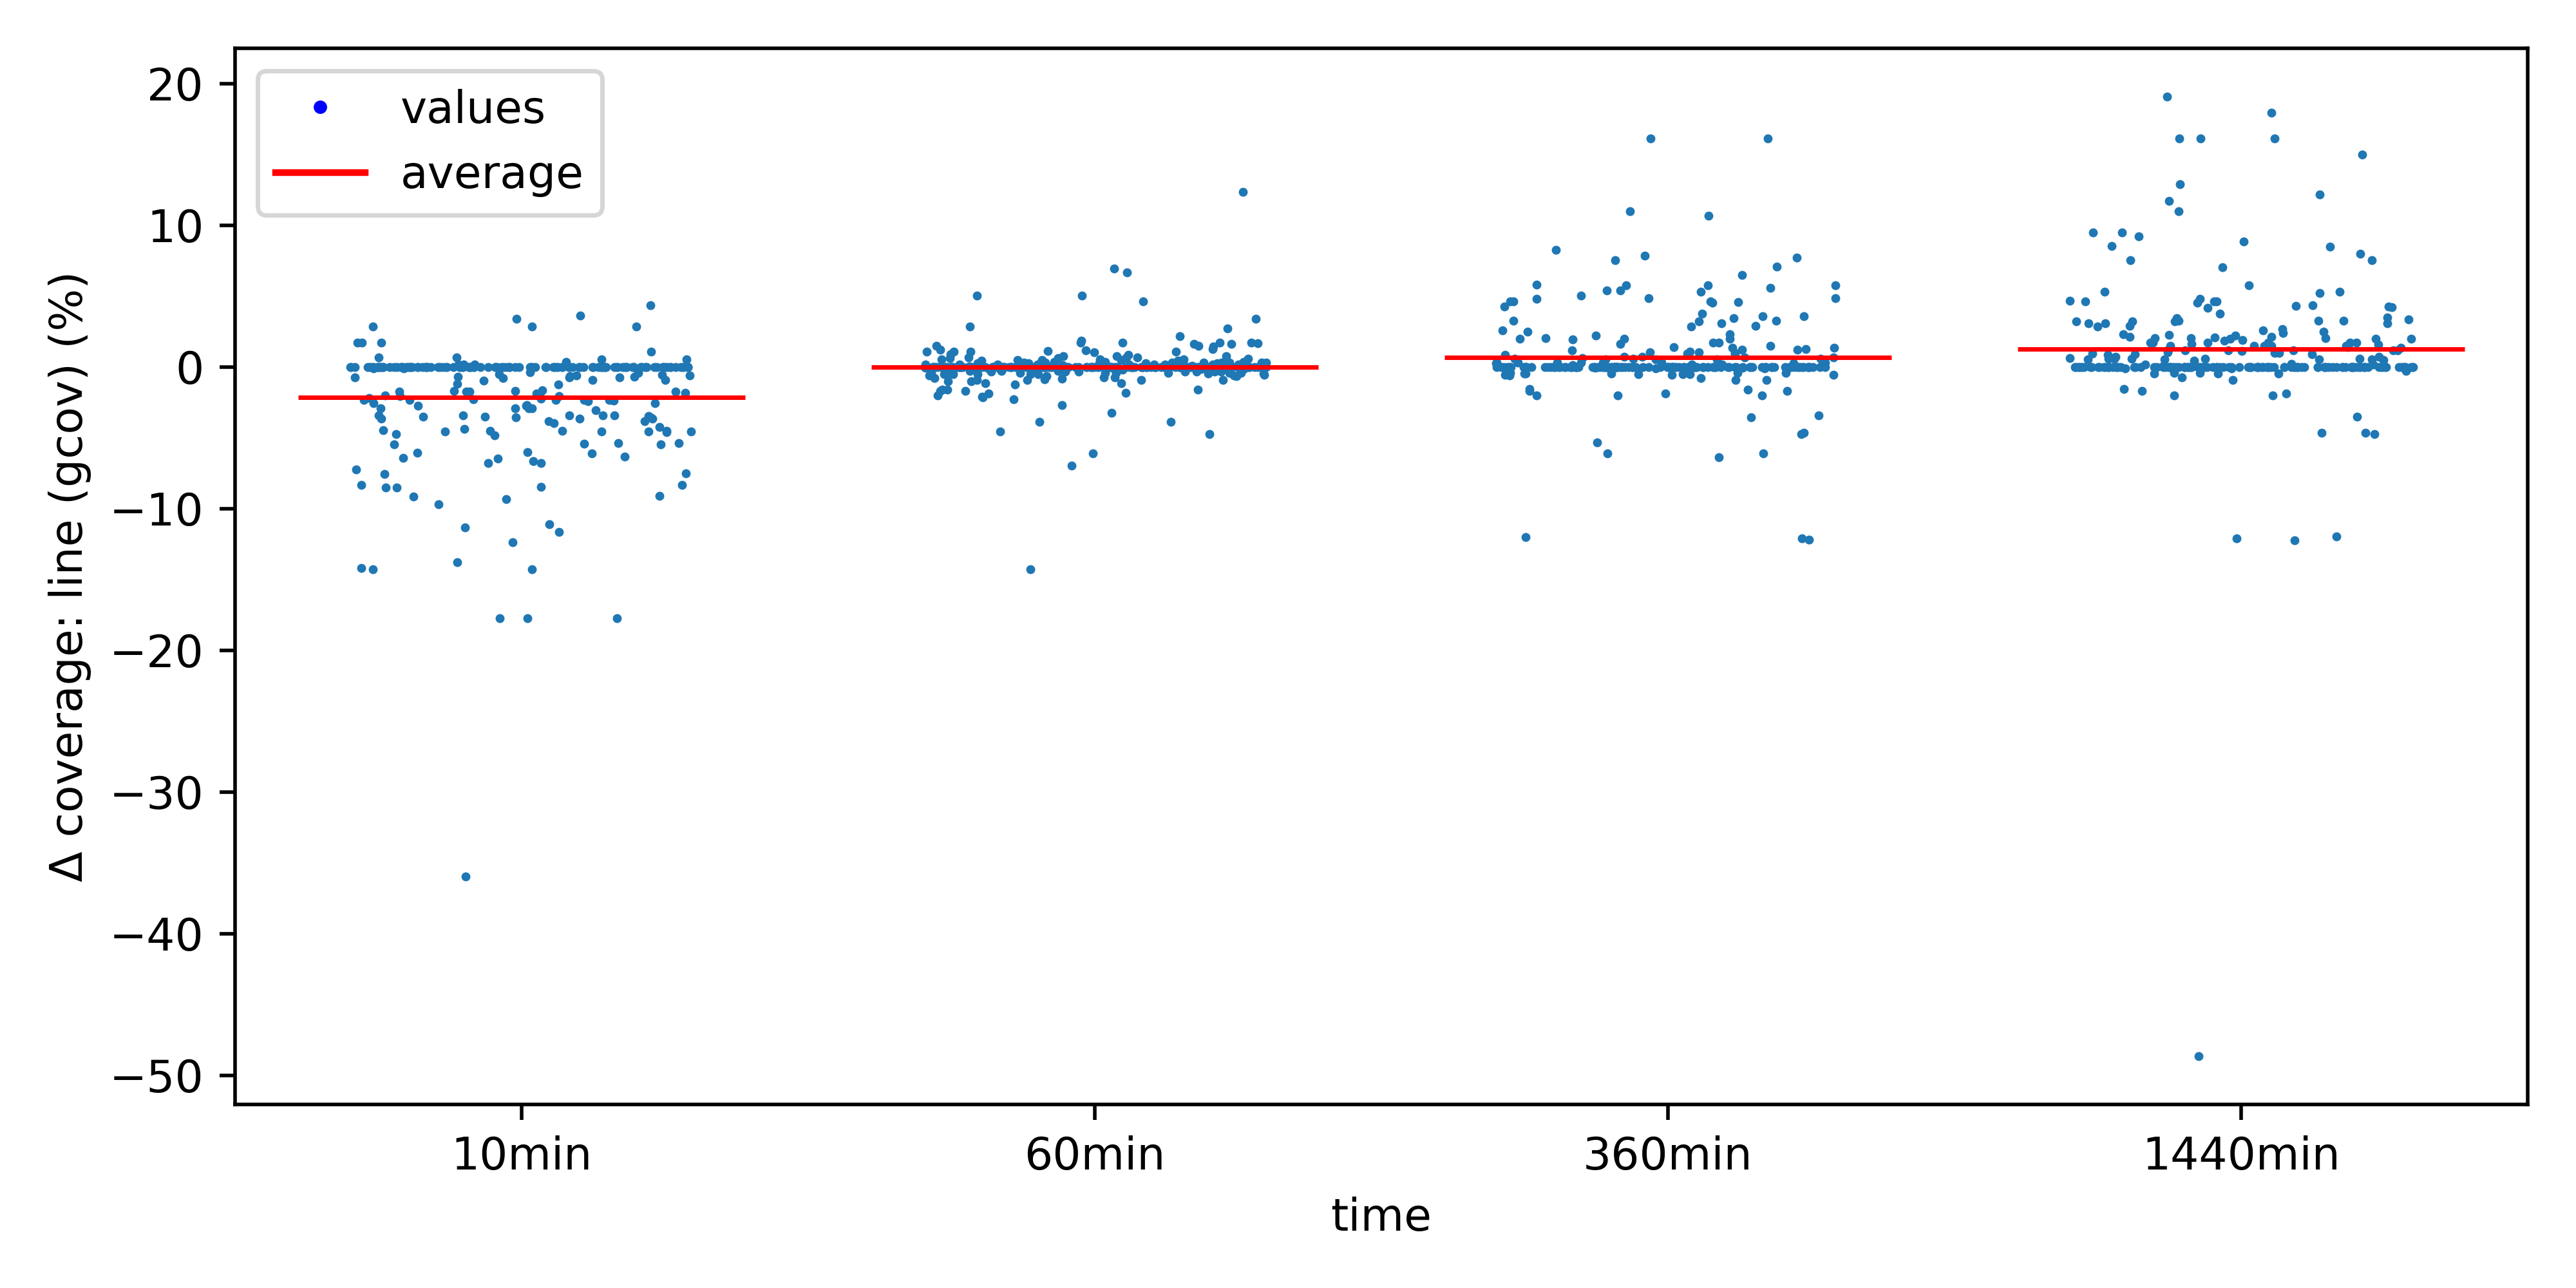
\includegraphics[width=0.8\textwidth]{../plots/gcov_cov/changes-by-time.png}
    \captionsetup{width=0.6\textwidth}
    \caption{Spread of coverage by run, normalized to the mean of the util at a timeout of 60 minutes, across different timeouts}
    \label{fig:spread_across_times_gcov}
\end{figure}

\subsubsection{Changes in Number of Errors}

Looking at changes in the number of errors in Figure~\ref{fig:spread_across_times_errors} paints an incomplete picture: While the number of errors increases with the additional analysis time, looking at the changes in individual utils shows that there exist no utils where no issues were found with more than one hour of analysis but where lower timeouts produced findings. There are utils where runs with longer timeouts only sometimes found the same number of errors as the one hour runs, which can be explained by overall variance in the test setup. There are multiple instances of utils where additional analysis time produced significantly more errors. As an example, the average number of total errors found in the util \lstinline{ptx} in one hour was 5. However, the runs with a timeout of 24 hours produced 16, 16, and 21 errors. For most utils however, as the figure suggests, the number of errors did not change based on timeouts.

\begin{figure}[ht]
    \centering
    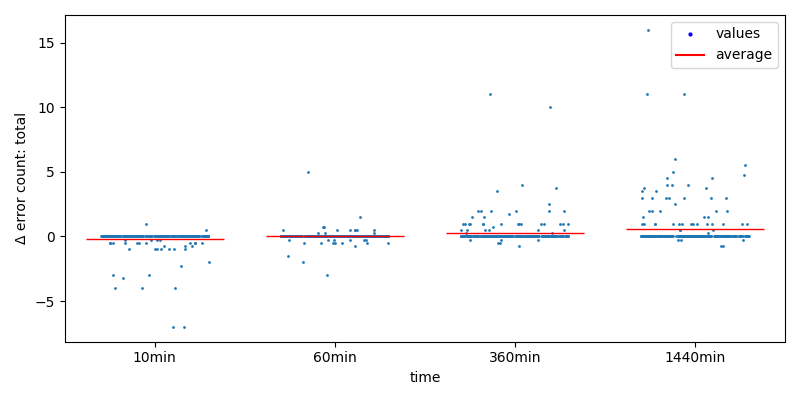
\includegraphics[width=0.8\textwidth]{../plots/num_errors (total)/changes-by-time.png}
    \captionsetup{width=0.6\textwidth}
    \caption{Spread of total number of errors found by run, normalized to the mean of the util at a timeout of 60 minutes, across different timeouts}
    \label{fig:spread_across_times_errors}
\end{figure}

\section{Testing More Recent Versions of coreutils}
\label{SoftwareEvolution}

As a second part, I wanted to see how the results from performing the same experiments on different versions of coreutils would behave. I chose two additional versions: 9.4, which is the current version at the time of the experiments, and 8.25, which was released exactly halfway between 6.10 and 9.4.

\subsection{Differences in Testing Setup}

The fundamental approach for the newer versions of coreutils remained the same: use old compilers on old systems where necessary and copy the binaries to KLEE's Docker image. Specifically, the following changes compared to the Dockerfile described in Section~\ref{Reproducing} were necessary:
\begin{itemize}
    \item For coreutils 8.25 Ubuntu 16.04 was chosen as the base image according to the same logic described in Section~\ref{LLVM}. Similarly, Ubuntu 22.04 was chosen for coreutils 9.4, since KLEE requires at most LLVM 13 and Ubuntu 24.04 (which is the latest available LTS version available) no longer supports a version of LLVM compatible with KLEE.
    \item The step replacing parts of the source code of \lstinline{sort.c}, as described in\cite{KLEEFAQ}, was changed from replacing \lstinline{(128 * 1024)} with \lstinline{(1024)} (compared to from \lstinline{(1024 * 1024)} to \lstinline{1024} in coreutils 6.10) in both coreutils 8.25 and 9.4, since the source code was changed in the meantime.
    \item For coreutils 8.25, LLVM and clang need to be installed at version 3.5, for coreutils at version 13.
    \item For coreutils 8.25, pip needed to be upgraded to version 19, because otherwise a python incompatibility prevented the installation of WLLVM.
    \item For coreutils 8.25, the WLLVM version remained unchanged compared to 6.10, but version 1.3.1 was chosen for coreutils 9.4.
    \item The \lstinline{configure} step when building both coreutils 8.25 and 9.4 requires an environment variable to run as root (which is the default user of Ubuntu's Docker images).
    \item Finally, the optimization flags for the LLVM bytecode generation step needed to be changed. According to the documentation, while just using \lstinline{-O0} on its own is fine for LLVM 3.4 (which is what is used for coreutils 6.10), this is no longer recommended for more recent versions.\cite{KLEETutorial,KLEEIssue} However, I could not get the compiler to build coreutils 8.25 using the proposed solution of \lstinline{-O1 -Xclang -disable-llvm-passes}. Specifically, I needed to remove the \lstinline{-Xclang} argument to get the build stage to complete successfully.
\end{itemize}

\subsection{Findings}

I chose a fixed timeout of 60 minutes as a constant to compare the different versions of coreutils. I then executed three runs of each additional version.

\subsubsection{Changes in Coverage}

Figure~\ref{fig:spread_across_versions_gcov} shows the coverage changes measured. The results indicate that the variance compared to version 6.10 predictively increases between the versions, as the code incrementally changes. Certain utils seem to become better penetrable by KLEE, while the coverage of others decreases, at times catastrophically. The overall average decreases across versions, which could be explained by increased complexity in the software as features are added.

\begin{figure}[ht]
    \centering
    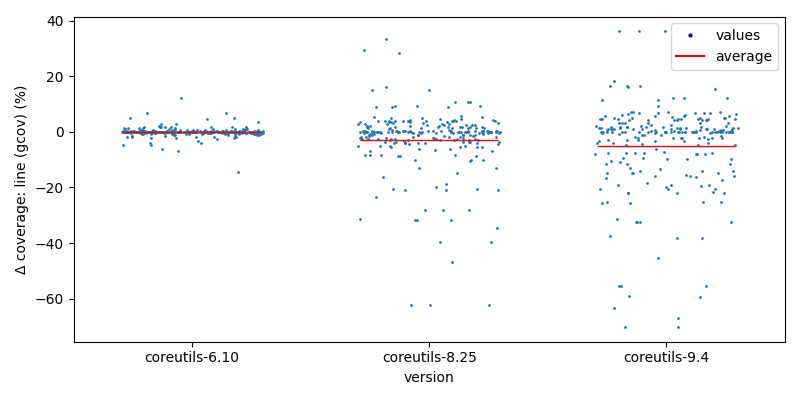
\includegraphics[width=0.8\textwidth]{../plots/gcov_cov/changes-by-version.png}
    \captionsetup{width=0.6\textwidth}
    \caption{Spread of coverage by run, normalized to the mean of the util at version 6.10, across different versions}
    \label{fig:spread_across_versions_gcov}
\end{figure}


\subsubsection{Changes in Number of Errors}

The number of errors found by KLEE remains fairly constant across the software versions and seems to even increase slightly for version 9.4. This is surprising to me, as the number of software errors should ideally decrease with time as bugs are fixed. However, this effect might be mitigated by new code adding new features or adapting the software to a changing environment introducing new errors. It might also show that running off-the-shelf fuzzing tools can be a path to finding undiscovered errors in software systems.

However, this speculation is difficult to maintain in the face of my inability to crash any util by manually replaying the inputs created by \lstinline{ktest-tool} for a sample of errors reported on version 9.4. This would indicate that many (if not all) of the reported errors are in fact false positives. However, to draw definitive conclusions about this, one would need to go through every error reported and manually check them. And, as argued in Section~\ref{Timeouts}, this could not be done as part of this project.

\begin{figure}[ht]
    \centering
    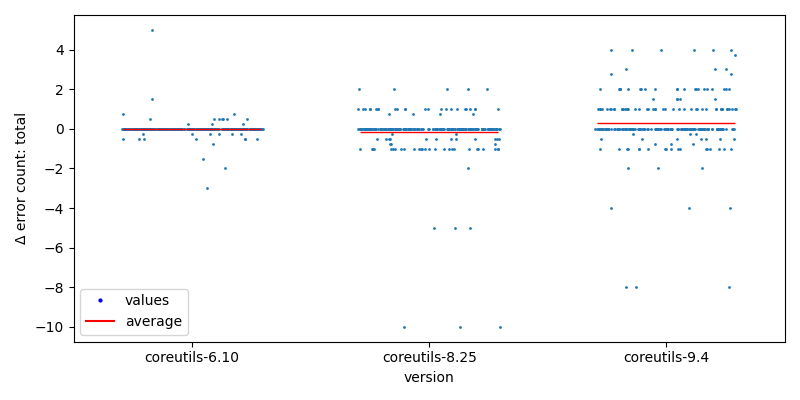
\includegraphics[width=0.8\textwidth]{../plots/num_errors (total)/changes-by-version.png}
    \captionsetup{width=0.6\textwidth}
    \caption{Spread of total number of errors found by run, normalized to the mean of the util at version 6.10, across different versions}
    \label{fig:spread_across_version_errors}
\end{figure}


\section{Discussion}
\subsection{Research Questions}

Section~\ref{Reproducing} showed that it is possible to run the current version of KLEE on coreutils 6.10, even though it requires multiple assembly steps across different Docker images to resolve version incompatibilities. The original paper provided two forms of measurements: coverage as reported by \lstinline{gcov} on executable lines of code and number of errors. Examining the specific errors found by KLEE is too complex and big a task to be included in this project. In the face of this, I opted to using the number of errors as an easier to calculate if inaccurate proxy.

Section~\ref{Timeouts} goes into further detail on the variance between test runs. It then continues by contrasting the results reported by the original KLEE paper with the results measured in the experiments done during this project. For code coverage, my test results were similar to what was reported by \citeauthor{KLEE}, validating the experiments. However, there still remain unexplained minor differences. Finally, the influence of different timeouts on the results is examined. Additional analysis time predictively leads to an increased coverage and number of errors found.

Section~\ref{SoftwareEvolution} discusses the results of the same experiment on different versions of coreutils. It introduces the changes necessary to run the test suite built in this project on versions 8.25 and 9.4. The results show a slightly decreasing code coverage with increased version number and a steady number of errors found. However, it also discusses how those errors might be largely false positives.

\subsection{Produced Artifacts}
\subsection{Future Work}

\clearpage
% \columnbreak
\defbibheading{bibliography}[\bibname]{\section*{#1}}
\addcontentsline{toc}{section}{\bibname}
\printbibliography

\renewcommand{\thesubsection}{\arabic{subsection}}
\renewcommand{\thesubsubsection}{\arabic{subsection}.\arabic{subsubsection}}
\setcounter{subsection}{0}
\setcounter{subsubsection}{0}
\section*{Appendix}
\addcontentsline{toc}{section}{Appendix}
\subsection{Building coreutils 6.10 on KLEE's Docker image}
\label{AppendixErrorBuildOldInNew}
\subsubsection{Error}
\lstinputlisting[firstline=1130, consecutivenumbers=false]{assets/build-coreutils-6.10-on-klee-image.txt}
\subsubsection{\texorpdfstring{\lstinline{freadahead.c}}{freadahead.c}}
The license has been cut for brevity's sake.
\lstinputlisting[firstline=17, language=C, consecutivenumbers=false]{assets/freadahead.c}
\end{document}
